\documentclass[conference]{IEEEtran}
%\documentclass[conference,draftcls]{IEEEtran}



% *** CITATION PACKAGES ***
%
%\usepackage{cite}
% cite.sty was written by Donald Arseneau
% V1.6 and later of IEEEtran pre-defines the format of the cite.sty package
% \cite{} output to follow that of IEEE. Loading the cite package will
% result in citation numbers being automatically sorted and properly
% "compressed/ranged". e.g., [1], [9], [2], [7], [5], [6] without using
% cite.sty will become [1], [2], [5]--[7], [9] using cite.sty. cite.sty's
% \cite will automatically add leading space, if needed. Use cite.sty's
% noadjust option (cite.sty V3.8 and later) if you want to turn this off.
% cite.sty is already installed on most LaTeX systems. Be sure and use
% version 4.0 (2003-05-27) and later if using hyperref.sty. cite.sty does
% not currently provide for hyperlinked citations.
% The latest version can be obtained at:
% http://www.ctan.org/tex-archive/macros/latex/contrib/cite/
% The documentation is contained in the cite.sty file itself.






% *** GRAPHICS RELATED PACKAGES ***
%
\ifCLASSINFOpdf
  \usepackage[pdftex]{graphicx}
  % declare the path(s) where your graphic files are
  % \graphicspath{{../pdf/}{../jpeg/}}
  % and their extensions so you won't have to specify these with
  % every instance of \includegraphics
  % \DeclareGraphicsExtensions{.pdf,.jpeg,.png}
\else
  % or other class option (dvipsone, dvipdf, if not using dvips). graphicx
  % will default to the driver specified in the system graphics.cfg if no
  % driver is specified.
  \usepackage[dvips]{graphicx}
  % declare the path(s) where your graphic files are
  % \graphicspath{{../eps/}}
  % and their extensions so you won't have to specify these with
  % every instance of \includegraphics
  \DeclareGraphicsExtensions{.eps}
\fi
% graphicx was written by David Carlisle and Sebastian Rahtz. It is
% required if you want graphics, photos, etc. graphicx.sty is already
% installed on most LaTeX systems. The latest version and documentation can
% be obtained at: 
% http://www.ctan.org/tex-archive/macros/latex/required/graphics/
% Another good source of documentation is "Using Imported Graphics in
% LaTeX2e" by Keith Reckdahl which can be found as epslatex.ps or
% epslatex.pdf at: http://www.ctan.org/tex-archive/info/
%
% latex, and pdflatex in dvi mode, support graphics in encapsulated
% postscript (.eps) format. pdflatex in pdf mode supports graphics
% in .pdf, .jpeg, .png and .mps (metapost) formats. Users should ensure
% that all non-photo figures use a vector format (.eps, .pdf, .mps) and
% not a bitmapped formats (.jpeg, .png). IEEE frowns on bitmapped formats
% which can result in "jaggedy"/blurry rendering of lines and letters as
% well as large increases in file sizes.
%
% You can find documentation about the pdfTeX application at:
% http://www.tug.org/applications/pdftex



\setlength{\parskip}{0.05cm}



% *** MATH PACKAGES ***
%
\usepackage[cmex10]{amsmath}
\usepackage{amssymb}
% A popular package from the American Mathematical Society that provides
% many useful and powerful commands for dealing with mathematics. If using
% it, be sure to load this package with the cmex10 option to ensure that
% only type 1 fonts will utilized at all point sizes. Without this option,
% it is possible that some math symbols, particularly those within
% footnotes, will be rendered in bitmap form which will result in a
% document that can not be IEEE Xplore compliant!
%
% Also, note that the amsmath package sets \interdisplaylinepenalty to 10000
% thus preventing page breaks from occurring within multiline equations. Use:
\interdisplaylinepenalty=2500
% after loading amsmath to restore such page breaks as IEEEtran.cls normally
% does. amsmath.sty is already installed on most LaTeX systems. The latest
% version and documentation can be obtained at:
% http://www.ctan.org/tex-archive/macros/latex/required/amslatex/math/

\usepackage{color}



% *** SPECIALIZED LIST PACKAGES ***
%
%\usepackage{algorithmic}
% algorithmic.sty was written by Peter Williams and Rogerio Brito.
% This package provides an algorithmic environment fo describing algorithms.
% You can use the algorithmic environment in-text or within a figure
% environment to provide for a floating algorithm. Do NOT use the algorithm
% floating environment provided by algorithm.sty (by the same authors) or
% algorithm2e.sty (by Christophe Fiorio) as IEEE does not use dedicated
% algorithm float types and packages that provide these will not provide
% correct IEEE style captions. The latest version and documentation of
% algorithmic.sty can be obtained at:
% http://www.ctan.org/tex-archive/macros/latex/contrib/algorithms/
% There is also a support site at:
% http://algorithms.berlios.de/index.html
% Also of interest may be the (relatively newer and more customizable)
% algorithmicx.sty package by Szasz Janos:
% http://www.ctan.org/tex-archive/macros/latex/contrib/algorithmicx/




% *** ALIGNMENT PACKAGES ***
%
%\usepackage{array}
% Frank Mittelbach's and David Carlisle's array.sty patches and improves
% the standard LaTeX2e array and tabular environments to provide better
% appearance and additional user controls. As the default LaTeX2e table
% generation code is lacking to the point of almost being broken with
% respect to the quality of the end results, all users are strongly
% advised to use an enhanced (at the very least that provided by array.sty)
% set of table tools. array.sty is already installed on most systems. The
% latest version and documentation can be obtained at:
% http://www.ctan.org/tex-archive/macros/latex/required/tools/


%\usepackage{mdwmath}
%\usepackage{mdwtab}
% Also highly recommended is Mark Wooding's extremely powerful MDW tools,
% especially mdwmath.sty and mdwtab.sty which are used to format equations
% and tables, respectively. The MDWtools set is already installed on most
% LaTeX systems. The lastest version and documentation is available at:
% http://www.ctan.org/tex-archive/macros/latex/contrib/mdwtools/


% IEEEtran contains the IEEEeqnarray family of commands that can be used to
% generate multiline equations as well as matrices, tables, etc., of high
% quality.


%\usepackage{eqparbox}
% Also of notable interest is Scott Pakin's eqparbox package for creating
% (automatically sized) equal width boxes - aka "natural width parboxes".
% Available at:
% http://www.ctan.org/tex-archive/macros/latex/contrib/eqparbox/





% *** SUBFIGURE PACKAGES ***
%\usepackage[tight,footnotesize]{subfigure}
% subfigure.sty was written by Steven Douglas Cochran. This package makes it
% easy to put subfigures in your figures. e.g., "Figure 1a and 1b". For IEEE
% work, it is a good idea to load it with the tight package option to reduce
% the amount of white space around the subfigures. subfigure.sty is already
% installed on most LaTeX systems. The latest version and documentation can
% be obtained at:
% http://www.ctan.org/tex-archive/obsolete/macros/latex/contrib/subfigure/
% subfigure.sty has been superceeded by subfig.sty.



%\usepackage[caption=false]{caption}
%\usepackage[font=footnotesize]{subfig}
% subfig.sty, also written by Steven Douglas Cochran, is the modern
% replacement for subfigure.sty. However, subfig.sty requires and
% automatically loads Axel Sommerfeldt's caption.sty which will override
% IEEEtran.cls handling of captions and this will result in nonIEEE style
% figure/table captions. To prevent this problem, be sure and preload
% caption.sty with its "caption=false" package option. This is will preserve
% IEEEtran.cls handing of captions. Version 1.3 (2005/06/28) and later 
% (recommended due to many improvements over 1.2) of subfig.sty supports
% the caption=false option directly:
%\usepackage[caption=false,font=footnotesize]{subfig}
%
% The latest version and documentation can be obtained at:
% http://www.ctan.org/tex-archive/macros/latex/contrib/subfig/
% The latest version and documentation of caption.sty can be obtained at:
% http://www.ctan.org/tex-archive/macros/latex/contrib/caption/




% *** FLOAT PACKAGES ***
%
%\usepackage{fixltx2e}
% fixltx2e, the successor to the earlier fix2col.sty, was written by
% Frank Mittelbach and David Carlisle. This package corrects a few problems
% in the LaTeX2e kernel, the most notable of which is that in current
% LaTeX2e releases, the ordering of single and double column floats is not
% guaranteed to be preserved. Thus, an unpatched LaTeX2e can allow a
% single column figure to be placed prior to an earlier double column
% figure. The latest version and documentation can be found at:
% http://www.ctan.org/tex-archive/macros/latex/base/



%\usepackage{stfloats}
% stfloats.sty was written by Sigitas Tolusis. This package gives LaTeX2e
% the ability to do double column floats at the bottom of the page as well
% as the top. (e.g., "\begin{figure*}[!b]" is not normally possible in
% LaTeX2e). It also provides a command:
%\fnbelowfloat
% to enable the placement of footnotes below bottom floats (the standard
% LaTeX2e kernel puts them above bottom floats). This is an invasive package
% which rewrites many portions of the LaTeX2e float routines. It may not work
% with other packages that modify the LaTeX2e float routines. The latest
% version and documentation can be obtained at:
% http://www.ctan.org/tex-archive/macros/latex/contrib/sttools/
% Documentation is contained in the stfloats.sty comments as well as in the
% presfull.pdf file. Do not use the stfloats baselinefloat ability as IEEE
% does not allow \baselineskip to stretch. Authors submitting work to the
% IEEE should note that IEEE rarely uses double column equations and
% that authors should try to avoid such use. Do not be tempted to use the
% cuted.sty or midfloat.sty packages (also by Sigitas Tolusis) as IEEE does
% not format its papers in such ways.





% *** PDF, URL AND HYPERLINK PACKAGES ***
%
%\usepackage{url}
% url.sty was written by Donald Arseneau. It provides better support for
% handling and breaking URLs. url.sty is already installed on most LaTeX
% systems. The latest version can be obtained at:
% http://www.ctan.org/tex-archive/macros/latex/contrib/misc/
% Read the url.sty source comments for usage information. Basically,
% \url{my_url_here}.



% *** Do not adjust lengths that control margins, column widths, etc. ***
% *** Do not use packages that alter fonts (such as pslatex).         ***
% There should be no need to do such things with IEEEtran.cls V1.6 and later.
% (Unless specifically asked to do so by the journal or conference you plan
% to submit to, of course. )


% correct bad hyphenation here
\hyphenation{op-tical net-works semi-conduc-tor}

\newcommand\numberthis{\stepcounter{equation}\tag{\theequation}}
\newcommand{\m}[1]{\mathbf{#1}^m}

\begin{document}
%
% paper title
% can use linebreaks \\ within to get better formatting as desired
\title{Some thought experiments on the applicability of Granger causality and Directed Information in inferring direction of information flows}
\author{Praveen Venkatesh and Pulkit Grover\\Carnegie Mellon University}

% make the title area
\maketitle

% Abstract --------------------------------------------------------------------

\begin{abstract}
	Granger causality is an established measure of the ``causal influence'' that one stochastic process has on another. Along with its more recent generalization -- Directed Information -- Granger Causality has been used extensively in neuroscience, and in complex interconnected systems in general, to infer causal influences. Of late, many works have begun to interpret the direction of causal influence as the direction of ``information flow'', which to us appears to be a questionable extrapolation {\color{red}(the question we raise is akin to, but different from, a criticism of Granger Causality that compares it to true causality, as defined by Judea Pearl)}. We test whether these measures correctly predict the direction of information flow by using two simple theoretical experiments, in which the true direction of information flow is known by design. The experiments are based on a communication system with a feedback channel, upon which a strategy inspired by the work of Schalkwijk and Kailath is employed. We show that in these experiments, the direction of information flow can be opposite to that which is inferred using Granger causality and Directed Information. Thus, while it might be reasonable to infer the direction of causal influence using these techniques, one needs to exercise care in interpreting the direction of causal influence as the direction of information flow.
\end{abstract}

\IEEEpeerreviewmaketitle

% Introduction ----------------------------------------------------------------

\section{Introduction}
\label{sec:intro}

% Intro: Motivation -----------------------------------------------------------

\subsection{Motivation}
\label{sec:motivation}

This work is in large part motivated by a recent surge of interest in understanding neural circuits -- the connectivity and dynamic activity of different regions of the brain -- and how they give rise to behavior and experience. This is evidenced by the launching of the BRAIN initiative in the US and the Human Brain Project in Europe. To quote from \emph{BRAIN 2025: A Scientific Vision}\footnote{The BRAIN Working Group's report to the Advisory Committee to the Director of the NIH}, we wish to ``map connected neurons in local circuits and distributed brain systems, enabling an understanding of the relationship between neuronal structure and function'', clearly indicating the move towards understanding (a) the connectivity and (b) the computational function of different brain regions. While the question of how the brain computes has been of immense interest for several decades, only recently have measurement techniques become sophisticated enough to be able to simultaneously record the activity of multiple neurons, or multiple neural populations.

In order to understand how the brain performs computations, it could be useful to first understand the directions of \emph{information flow} in various parts of the brain (e.g.~\cite{blinowska2004granger,dhamala2008analyzing,nolte2008robustly,korzeniewska2003determination,schippers2010mapping} etc.). In an effort to make headway on the goals of \emph{BRAIN 2025}, several works use Granger causality (and less often, its information-theoretic generalization -- Directed Information) to understand how this information flows (eg.~\cite{Brovelli2004BetaOscillations,goebel2003investigating,deshpande2008effective}), or to acquire directed maps of functional connectivity (eg.~\cite{friston2013analysing,goebel2003investigating,deshpande2008effective}). For instance, in~\cite{Brovelli2004BetaOscillations}, Granger causal influences that are measured between somatosensory and motor sites are said to ``support the idea that somatosensory feedback provides information to the sensorimotor system that is used to control motor output''. This raises the question: do these directed connectivity maps, as determined by directional causal influence measures such as Granger causality, correctly identify the directions along which information flows in the brain?

% Intro: How GC is used in neuroscience today ---------------------------------

\subsection{How Granger Causality is used in Neuroscience today}
\label{sec:gc-used-in-neuroscience}

Several works have outlined the procedures involved in using Granger Causality to estimate causal influences in the brain (\cite{bernasconi2000bidirectional,Brovelli2004BetaOscillations,Ding2000ShortWindow,Roebroeck2005MappingDirected,Bressler2011WienerGranger,Barnett2014MVGC,Ding2006GrangerCausality}). Here, we briefly describe how Granger Causal influence is quantified, and how it is computed in these works.

Granger causality, as originally described by Granger~\cite{Granger1969InvestigatingCausal}, measures the level of influence that one process $\{X\}$ has on another process $\{Y\}$. The analysis compares the \emph{error in predicting} the $\{Y\}$ process based on (i) simply the past of $\{Y\}$, and (ii) based on the past of both $\{X\}$ and $\{Y\}$. The Granger causality metric is the ratio of these errors, encapsulating the innovations that the process $\{X\}$ causally supplies to the process $\{Y\}$. Many variations of Granger causality have also been considered, including a generalization -- Directed Information (see~\cite{MasseyCausality,quinn,weissman}) -- an information-theoretic quantity denoted by $I(\m{X}\to\m{Y})$. These form possible alternatives for estimating the direction of causal influence, but Directed Information is a generalization of many of these metrics~\cite{quinn}.

The computation of Granger causality, in general, requires that the processes under consideration be stationary. In neuroscientific experiments, this is usually not the case, as the express objective of the experiment is to understand brain function while the brain is subjected to a task. Typically, data analysis techniques either assume stationarity regardless, or circumvent the problem by working with time-windows short enough that the processes \emph{are} in fact stationary within those windows~\cite{Ding2000ShortWindow}. In the latter case, Granger causal influences are computed for each window individually, in order to produce a dynamic description of brain connectivity as the brain carries out the said task. The Granger Causality metrics can be accurately computed even for short time windows, because neuroscientific experiments usually have multiple trials, i.e.\ multiple realizations of the same processes, allowing for fitting regression coefficients accurately~\cite{Ding2000ShortWindow}.

In order to determine the direction of causal influence, the Granger Causality metric (ratio of residual variances) from $\{X\}$ to $\{Y\}$ is \emph{compared} to that from $\{Y\}$ to $\{X\}$. The direction of causal influence is taken to be the direction with a greater Granger Causality metric. Further, this direction of causal influence is interpreted to be the direction of informationf flow -- the interpretation we question in this paper. We also note that many of these works use a spectral version of Granger Causality, that supplies this metric as a function of frequency. It then becomes possible to also determine the brain wave frequency at which these influences occur. However, we restrict our analysis to the simpler non-spectral version of Granger Causality, since it is sufficient to for the purpose of our arguments.

We note here that Granger's original analysis does not compare this metric on forward and reverse links, however, this appears to be commonly done in practice. {\color{red} TODO: Cite Tsachy's paper here.}

While we accept that Granger Causal influence can be accurately computed (provided measurements are taken suitably; see Section~\ref{sec:previous-criticisms-of-gc}) and can be useful in many situations (see Section~\ref{sec:discussion}), interpreting the direction of Granger Causal influence as the direction of information flow can be erroneous, as we demonstrate in this paper.

% Intro: Previous criticisms of GC --------------------------------------------

\subsection{A short survey of previous criticisms of Granger Causality}
\label{sec:previous-criticisms-of-gc}

Several objections have been leveled against Granger Causality in the past. We give, here, a short overview of these and describe why our objection is novel, and possibly more fundamental in nature, at least in the context of its usage in neuroscience.

\begin{enumerate}
	\item First, Granger Causality suffers from what we call the ``hidden node problem''. If two observed nodes receive causal influences from a third, latent node, then a causal influence may be detected between the observed nodes, even if they are independent of each other~\cite{pearl2009causality-hidden-node}. All nodes need to be observed, therefore, to avoid finding spurious influences.
	\item Second, if the measurements from each node are differentially affected by noise, then the predicted direction of causal influence might be opposite to the true direction (\cite{nalatore2007mitigating,andersson2005testing}). Measurements need to be relatively noiseless and precise in order to obtain the correct direction of causal influece.
	\item Third, subsampling the processes can produce misleading Granger Causal relations~\cite{gong2015discovering}. Performing Granger Causal analysis on subsampled time series can lead one to miss the causal influence. If pre-processing involves subsampling, then this should be done with care.
\end{enumerate}

It is important to note that the technical objections listed above are all concerned with \emph{measurement}. They indicate that incorrect Granger Causal influences may be computed if there is some deficiency in the measurement procedure. These objections can be resolved by taking better measurements (by sampling more nodes, with higher signal-to-noise ratio, etc.).

Our objection, on the other hand, is much more fundamental. \emph{Even if} the measurements are made with infinite accuracy, and the regression coefficients associated with computing Granger Causality are precisely estimated, and the Granger Causality metric is perfectly computed (as is the case in our counter-examples), Granger Causal influence would \emph{still} not give the correct direction of information flow. To our knowledge, this is a completely novel argument against Granger Causality, and one that is far more serious than previous objections, at least as far as its usefulness in understanding brain function is concerned.

% Intro: Our counter-examples -------------------------------------------------

\subsection{Our counter-examples and our main result}
\label{sec:our-counterexamples}

This paper considers two experiments (introduced in Section~\ref{sec:sk}) where a transmitter $Tx$ wants to communicate a message to a receiver $Rx$ in presence of a feedback channel (in one experiment, the feedback link is noiseless, while in the other it is noisy). We assume that the experimenter is able to record the transmissions of $Tx$ and $Rx$ using some probing mechanism. Provided with these measurements, the experimenter wants to estimate the direction of information flow, which in this context is the direction of flow of the message. Our results, derived in Section~\ref{sec:analytical-results} and numerically illustrated in Section~\ref{sec:numerical-results}, show that both Granger causality and Directed Information can incorrectly estimate the direction of information flow. The first experiment considers the (unrealistic) case of communication across noiseless feedback channels. The second experiment allows for noise in the feedback channel. In both cases, linear strategies inspired from the scheme of Schalkwijk and Kailath~\cite{S&K} are used.

Our goal here is to bring out the point that whether Granger causality and Directed Information can be used to interpret direction of information flows is an issue that can be, and perhaps should be, considered using thought experiments on simple communication problems where \emph{information flow direction, and quantity, is already known}. If the direction of causal influence yielded by Granger causality or some other similar measure were to match the known direction of information flow, then that measure can be more confidently used in experiments. While our results strongly suggest that one needs to exercise care in interpreting Granger causality and Directed Information dominance as an indicator for the direction of information flow, there are several shortcomings that need to be addressed in order to understand the issue at depth. These shortcomings are discussed in detail in Section~\ref{sec:objections-and-shortcomings}.

% Intro: Possible objections and shortcomings ---------------------------------

\subsection{Possible objections to, and shortcomings of this work}
\label{sec:objections-and-shortcomings}

A review of a previous submission raised some objections to this work, which we seek to clarify here. Further, our analysis has certain shortcomings, which we acknowledge. These could form the basis for future work.

\begin{enumerate}
	\item Firstly, and most importantly, previous work has already shown that presence of a Granger Causal influence does not imply true causation. Judea Pearl classifies Granger Causality as stemming from a ``statistical'' model, rather than from a ``causal'' model~\cite{pearl2009causality-gc-stat}. A potential issue, therefore, might be the question the novelty of this work, given that Pearl's classification could be seen to clear up the misconception. While our argument is, in spirit, very similar to this criticism of Granger causality, in the situation we study, we ask a different question - we wish to understand whether or not Granger Causality gives the correct direction of \emph{information flow}. Further, we give a concrete counter-example in this context, which is very relevant in the modern neuroscience setting.
	\item It might appear that we make a circular argument while computing the Granger Causal influences in our counter-example, since we supply the model for the stochastic process and use the theoretical coeffiecients of the model directly to compute the Granger Causality metric. However, as we state in Section~\ref{sec:figure-it-out}, we assume that the regression coefficients of the Autoregressive model can be exactly estimated (even if the AR process is non-stationary), and discuss how this might be achieved with the help of multiple trials. {\color{red} (Move to conclusions?)}
	\item Our analysis does not tackle an information source that evolves with time. Hence, our communication process (inspired from the scheme of Schalkwijk and Kailath~\cite{S&K}) is non-ergodic. Since Granger causality is really just relative errors in prediction of a process, in presence or absence of knowledge of another process, we compute the obvious generalization of Granger causality to non-ergodic processes. Nevertheless, future work will address a situation with a linear dynamical system as the information source.
	\item Our experiments restrict themselves to Gaussian noise for simplicity, but neural spiking and spike-rate models for spikes tend to be very different from those used here. This is a clear direction for future work.
	\item The power and energy constraints are somewhat oversimplified to make the analysis simpler. This is for simplicity of exposition. A more general analysis is a trivial extension.
	\item We have also restricted ourselves to analyzing linear feedback communication strategies. In the presence of noise in the feedback link, linear communication strategies are known to be sub-optimal~\cite{YoungHanKimPaper}. In order to make a water-tight argument, we would need to show that Granger Causality fails to correctly predict the direction of information flow, even when an optimal communication strategy -- which would have to be non-linear. This could be scope for future work. However, we do not expect results to change dramatically -- when the feedback link is impaired by noise of only very low variance, the noiseless case should make for a good approximation of the system, and results should degrade gracefully, if there is any degradation at all.
	\item We consider a simple point-to-point network. In general networks, this issue could be even more complex. However, since this issue shows up even for the simplest network, we feel that the problem will only be exacerbated when the network is large.
	\item We would also like to note that this paper is \emph{not} mathematically deep. We believe that this is a strength of our analysis. Even simple counter-examples that do not employ difficult proof techniques are able to show that Granger Causality does not always correctly estimate the direction of information flow. {\color{red} (Move this, but where?)}
\end{enumerate}

\subsection{Discussion}
\begin{enumerate}
	\item \color{red} Some of this misconception might have arisen because of Massey's directed info conservation - we expect that dir info in the forward dirn goes up if the other one goes down - but this is a misnomer. (Do we still need this? I am increasingly of the opinion that directed info / GC capture nothing about the message)
\end{enumerate}

\section{ghgh}

This work is in large part motivated by a recent surge of interest in understanding neural circuits --- the connectivity and dynamic activity of parts of the brain --- and how they give rise to behavior and experience\footnote{This is evidenced in the launching of the BRAIN initiative in the US and the Human Brain Project in Europe.}. The question of how the brain computes has been of immense interest for several decades, but only recently have measurement techniques become sophisticated enough to be able to simultaneously record the activity of multiple neurons, or multiple neural populations.

In order to understand how the brain performs computations, it could be useful to understand first the direction of information flows  in various parts of the brain (e.g.~\cite{blinowska2004granger,dhamala2008analyzing,nolte2008robustly,korzeniewska2003determination,schippers2010mapping} etc.). For instance, what one might seek is a component-wise block diagram of the brain, where the brain is broken down into discrete computational units. In this picture, each computational unit receives information, processes it, and then passes it on to another unit.

In order to arrive at such an understanding of the brain, a natural method is to probe it to understand its functional connectivity\footnote{This is different from structural or anatomical connectivity in that links may sometimes be present, but not active.}. Analyses are then performed on the time series thus obtained from the probes, in order to say something about the functional connectivity -- which components influence each other, and which direction is this influence in. One commonly used analysis is based on the computation of Granger causality~\cite{Granger} with the measurements from each node. The Granger causality between two processes measures the level of influence that one process $\{X\}$ has on another process $\{Y\}$. The analysis compares the \textit{error in predicting} the $\{Y\}$ process based on (i) simply the past of $\{Y\}$, and (ii) based on the past of both $\{X\}$ and $\{Y\}$. Many variations of Granger causality have also been considered, including a generalization -- the Directed Information (see~\cite{MasseyCausality,quinn,weissman}) -- an information-theoretic quantity denoted by $I(\m{X}\to\m{Y})$. %So another strategy that could be used to infer causal influence of one process, e.g. $\{X\}$, on another process $\{Y\}$ is to estimate and compare $I(\m{X}\to\m{Y})$ and $I(\m{Y}\to\m{X})$ (normalized by $m$) in the limit of large $m$.

The question of when Granger causality is true causality has been hotly debated for quite some time (see, e.g.~\cite{jacobs1979difficulties} for some of the issues). Nevertheless, Granger causality is widely used for inferring causal influence in a wide variety of applications, ranging from biology to economics. In this work, we are more interested in a different issue on use of Granger causality (and Directed Information) that has received little attention: the interpretation of the dominant direction of causal influence as the direction of information flow. Quoting~\cite{nolte2008robustly} for instance, ``To understand interacting systems it is of fundamental importance to distinguish the \emph{driver from the recipient}, and hence to be able to estimate the direction of information flow. The direction can be estimated with a temporal argument: the driver is earlier than the recipient implying that the driver contains information about the future of the recipient not contained in the past of the recipient while the reverse is not the case'' (emphasis has been added by us). Is the dominant direction of directed information really the direction of information flow? Can we assign communication labels of ``transmitter'' and ``receiver'' along the direction of directed information?

%Granger causality and Directed Information can, then, be used to estimate the direction of ``information flow'', and Granger causality often is. But in order to achieve an understanding of how the brain computes, it is necessary to think of the brain regions as communicating, as from a transmitter to a receiver. The authors of this paper believe that ascribing a direction to information flow in the brain, towards a goal of understanding how it computes, is meaningful only if there is also an implicit ``labelling'' of the brain regions being discussed as ``Trasmitter'' and ``Receiver''.

%In this paper, we question whether one is justified in assigning labels of ``Transmitter'' and ``Receiver'', based only on the activity we record from probes? 
%As one might anticipate, such an assignment can be a somewhat ambiguous for a system with feedback loops. 
This paper considers two experiments (introduced in Section~\ref{sec:sk}) where a transmitter $Tx$ wants to communicate a message to a receiver $Rx$ in presence of a feedback channel (in one experiment, the feedback link is noiseless, while in the other it is noisy). We assume that the experimenter is able to record the transmissions of $Tx$ and $Rx$ using some probing mechanism. Provided with these measurements, the experimenter wants to estimate which node is $Tx$ and which is $Rx$. Our results, derived in Section~\ref{sec:analytical-results} and numerically illustrated in Section~\ref{sec:numerical-results}, show that both Granger causality and Directed Information can incorrectly estimate which node is which. The first experiment is for the (unrealistic) case of communicating across noiseless feedback channels. The second experiment allows for noise in the feedback channel as well. In both cases, linear strategies inspired from the strategy of Schalkwijk and Kailath~\cite{S&K} are used.

Our goal here is to bring out the point that whether Granger causality and Directed Information can be used to interpret direction of information flows is an issue that can be, and perhaps should be, considered using thought experiments on simple communication problems where \textit{information flow direction, and quantity, is already known}. If the prediction of Granger causality, or some other measure of information flow, matches with the known information flow, then that measure can be more confidently used in experiments. While our results strongly suggest that one needs to exercise care in interpreting Granger causality and Directed Information dominance as an indicator for the direction of information flow, there are several shortcomings that need to be addressed in order to understand the issue at depth. These shortcomings are discussed in detail in Section~\ref{sec:conclusions}.



%\begin{itemize}

%\item Motivation: Recent interest in understanding neural circuits, to understand how computation is being done -- the BRAIN initiative in the US and the Blue Brain (?) project for mapping the brain in Europe. The ultimate goal is to understand how the brain works, and potentially to use that to engineer better circuits and systems (if we can quote from either of the projects, even better!). Another motivation for this work is probing a circuit to understand how computation is being performed. Or probing a social network?

%\item Leads us to the tale of: What if a biologist came across a radio. How would they examine it? How will they probe it and based on the data, what conclusions will they draw? This has a circuit parallel as well. 

%\item The question of causality has been hotly debated elsewhere (see, e.g. ??). More recently, causality has come to be interpreted as the direction of information flows. We need as many citations for this as possible. Some of them: Korzeniewska2003 and papers that cite it. The more papers we can cite with info-flow directions in their title, the better.

%\item In communication parlance, information flows from the transmitter to the receiver. Feedback from the receiver can be viewed as information-flow as well. However, this flow could be of little intellectual interest [... why?...] %information flows not only from transmitter to receiver, but also on the feedback link in the reverse direction. Biological links, as well as circuits, tend to have substantial feedback, and thus it is of great interest to develop techniques to assign the ``transmitting'' and ``receiving'' nodes. 

%\item This paper performs some experiments on inferring the direction of information flows. To be able to ask the question of whether the information flow is predicted in the correct direction, we 

%\item The first experiment is for the case with noiseless feedback. In this highly asymmetric case, we observe that directed information and Granger causality can incorrectly predict the direction of forward and reverse links. 


%\end{itemize}

%Possible shortcomings of our approach/objections to our approach:
%\begin{itemize}
%\item The source is not an ergodic process. However, Granger causality is really just relative errors in prediction of a process, in presence or absence of knowledge of another process. So we compute the obvious generalization of Granger causality to non-ergodic processes. 
%\item In feedback communication channels, info flows not just from the transmitter to the receiver, but also from the receiver to the transmitter. So as long as the biologist does not make the leap from direction of information flow to assigning labels such as ``transmitter,'' and ``receiver,'' they will be fine. But if they do not assign these labels, how is computing direction of info flow helping them understand brain circuits? This is unclear to us. It could help them, for instance, to understand epileptic seizure propagation. But that provides little insight into computation (besides, that is really not ``info-flow'' at all!). 
%\item Directed information is computed for a Gaussian case. 
%\item Neural models for spikes tend to be very different from those used here. 
%\item Power and energy constraints are simplified.
%\item We consider a simple point-to-point network. In general networks, this issue could be even more complex.
%\item Granger's original analysis does not compare Granger causality on forward and reverse links. We are doing so, in part because it is often empirically done. Also, the ``conservation of directed information,'' an equality first derived by Massey~\cite{??}, could be viewed as suggesting that an increase in directed info in one direction must reduce it in the other direction. This is not true. For instance, making $X$ and $Y$ uncorrelated reduces directed info in both directions (and their sum) to zero. In other words, Massey's law is not a conservation law in the sense of conservations laws of energy, momentum, or mass, where the total energy/momentum/mass (\textit{i.e.}, the RHS) remains conserved (\textit{i.e.}, constant) regardless of the experiment performed on the entities. 
%\item More counterexamples need to be studied to get a better sense of when these tools are applicable and when they're not.
%\item The work that looks at noisy versions of observed transmissions already creates a concern on use of info flows. Our work bridges that work with info theory. Instead of being a one-off result, that work points to a deeper issue with use of directed info in interpreting info flows. 
%\end{itemize}



%Notes:

%You only seem to be assuming that the variance is $\sigma_\theta^2$. Nothing about whether it is a uniform random variable or something derived from quantizing a uniform random variable, or a Gaussian one. 

% --------------------------------------------------------------------------- %

\section{A simple feedback communication scheme}
\label{sec:sk}
This section summarizes the analysis in the work of Schalkwijk and Kailath~\cite{S&K}, and a simple (and previously known) extension to a noisy feedback case. It also establishes the model and the notation used in the paper.

The transmitter wants to convey a single zero-mean random number, $\Theta$, having variance
$\sigma_\theta^2$, to the receiver. $\Theta$ could be obtained, for instance, by quantizing a bounded interval on the real line (e.g. $[-1,1]$), as is done in the scheme of Schalkwijk and Kailath~\cite{S&K}. The forward channel is an AWGN channel with noise variance $\sigma_N^2$. We will use simple linear communication strategies for a noiseless feedback channel, as well as an AWGN feedback channel with noise variance $\sigma_R^2$. In both cases, the estimators will be shown to be unbiased and consistent (the error mean is zero, and the error variance converges to zero).

\subsection{Noiseless feedback: the Schalkwijk-Kailath strategy}
 In the first step, the transmitter sends\footnote{We assume that the power constraints are such that the scaling constant $\alpha$ in~\cite{S&K} is $1$.} $X_1 = \Theta$, which the receiver receives with added noise. The receiver sends back an estimate of $\Theta$ over the feedback link. In all subsequent iterations, the transmitter sends the receiver the error in its latest estimate.

Therefore, in general, the transmitter sends $X_i = \Theta - \widehat\Theta_{i-1}$ and the receiver receives $Y_i = X_i + N_i$, where $N_i \sim \mathcal{N}(0, \sigma_N^2)$ iid. The receiver then estimates $\widehat\Theta_i = \widehat\Theta_{i-1} + \frac{Y_i}{i}$, which results in:
\begin{align*}
	\widehat{\Theta}_{i}  &= \widehat{\Theta}_{i-1}+\frac{X_{i}+N_{i}}{i} \\
					  &= \widehat{\Theta}_{i-1}+\frac{\Theta-\widehat{\Theta}_{i-1}+N_{i}}{i} \\
					  &= \frac{(i-1)\widehat{\Theta}_{i-1}+\Theta+N_{i}}{i} \\
	i\widehat{\Theta}_{i} &= (i-1)\widehat{\Theta}_{i-1}+\Theta+N_{i} \\
					  &=(i-2)\widehat{\Theta}_{i-2}+\Theta+N_{i-1}+\Theta+N_{i} \\
					  & \qquad \vdots \\
					  &= i\Theta+\sum_{j=1}^{i}N_{j} \\
	\widehat{\Theta}_{i}  &=\Theta+\frac{1}{i}\sum_{j=1}^{i}N_{j} \numberthis \label{eq:theta_hat_i-noiseless}
\end{align*}

Through this scheme, the estimate $\widehat{\Theta}_{i}$ is seen to converge to $\Theta$ in mean-square sense as $i\rightarrow\infty$:
\begin{align*}
	\mathbb{E}[\widehat{\Theta}_{i}] &= \mathbb{E}\bigg[\Theta+\frac{1}{i}\sum_{j=1}^{i}N_{j}\bigg] = \mathbb{E}[\Theta]+0 \\
	\mathbb{E}[(\widehat{\Theta}_{i}-\Theta)^{2}] &= \mathbb{E}\bigg[\bigg(\frac{1}{i}\sum_{j=1}^{i}N_{j}\bigg)^{2}\bigg] \\
												  &= \frac{1}{i^{2}}\mathbb{E}\bigg[\bigg(\sum_{j=1}^{i}N_{j}\bigg)^{2}\bigg] = \frac{i}{i^{2}}\mathbb{E}[N_{1}^{2}] = \frac{\sigma_{N}^{2}}{i}\overset{i\to\infty}\longrightarrow 0.
\end{align*}

\subsection{Noisy feedback}
In the presence of noise in the feedback link, restricting our attention to linear strategies, we can use a simple modification of the Schalkwijk-Kailath strategy, incorporating the feedback\footnote{We note that implicitly, this strategy assumes an energy/SNR constraint on the feedback link. This is because the receiver simply sends back the estimate, which is shown to converge to the true value of $\Theta$.}. The receiver still simply transmits the estimate $\widehat{\Theta}_i$ based on the $i$-th forward channel output $Y_i=X_i+N_i$. The transmitter now receives corrupted versions $Z_i=\widehat\Theta_{i-1} + R_{i-1}$ of the receiver's transmissions. That is,
\begin{align*}
	\text{Transmitter's transmissions:}\;X_i &= \Theta - (\widehat\Theta_{i-1} + R_{i-1}) \\
	\text{Channel outputs at the receiver:}\;	Y_i &= X_i + N_i \\
	\text{Receiver's estimates \& transmissions:}\;	\widehat\Theta_i &= \widehat\Theta_{i-1} + \frac{Y_i}{i}
\end{align*}
where $R_{i-1}$ is the AWGN noise in the reverse link. $R_i \sim \mathcal{N}(0, \sigma_R^2)$ are iid random variables.

Linear strategies are known to be suboptimal for the communication problem~\cite{YoungHanKimPaper} (where $\Theta$ is a quantized random variable communicating a finite-rate message reliably), and for problems with non-classical information structures in general~\cite{Witsenhausen68}. Nevertheless, we now show that the resulting estimates $\widehat{\Theta}_i$  still converge to $\Theta$ in mean-square sense:
\begin{align*}
	i\widehat\Theta_i &= i\widehat\Theta_{i-1} + X_i + N_i \\
					  &= i\widehat\Theta_{i-1} + \Theta - \widehat\Theta_{i-1} - R_{i-1} + N_i \\
					  &= (i-1) \widehat\Theta_{i-1} + \Theta - R_{i-1} + N_i \numberthis \label{eq:theta_hat_i-noisy-once} \\
					  &\overset{(a)}{=} i\Theta + \sum_{k=1}^i N_k - \sum_{k=1}^{i-1} R_k \\
	\widehat\Theta_i  &= \Theta + \frac{1}{i} \sum_{k=1}^i N_k - \frac{1}{i} \sum_{k=1}^{i-1} R_k \numberthis \label{eq:theta_hat_i-noisy}
\end{align*}
where $(a)$ is obtained by expanding $\widehat{\Theta}_j$ recursively for $j=i-1,i-2,\ldots,2$. Therefore, the error in estimating $\Theta$ converges to $0$ in mean-square sense (\textit{i.e.}, $\widehat{\Theta}_i$ is a consistent estimate of $\Theta_i$ even in the presence of noise on the feedback link).

We also derive here an expression for $X_i$, which we will use later.
\begin{align*}
	X_i &= \Theta - \widehat\Theta_{i-1} - R_{i-1} \\
	&= \Theta - \bigg( \Theta + \frac{1}{i-1} \sum_{k=1}^{i-1} N_k - \frac{1}{i-1} \sum_{k=1}^{i-2} R_k \bigg) - R_{i-1} \\
	&= \frac{1}{i-1} \sum_{k=1}^{i-2} R_k - \frac{1}{i-1} \sum_{k=1}^{i-1} N_k - R_{i} \numberthis \label{eq:x_i-noisy}
\end{align*}

\section{Granger causality and directed information analyses for the strategies in Section~\ref{sec:sk}}
\label{sec:analytical-results}

\subsection{Granger causality for the noiseless feedback case}

Suppose we try to use the Granger causality measure of directed influence to infer the direction of information flow. As discussed in Section~\ref{sec:intro}, one might expect the direction of information flow --- and hence the direction of greater Granger causality --- to be from the transmitter to the receiver.

In order to compute the Granger causality in the reverse direction (from receiver to transmitter), we wish first to compute coefficients $\alpha_j$ such that:
\begin{equation*}
	X_i = \sum_{j=1}^{p}{\alpha_j X_{i-j}} + \epsilon_i
\end{equation*}
Note that $\alpha_j$ can themselves depend on $i$, since this is a non-stationary process (because the error $\Theta-\widehat{\Theta}_i = X_i$ converges to zero).
\begin{align*}
	X_i &= \Theta - \widehat\Theta_{i-1} \\
		&= \Theta - \big( \widehat\Theta_{i-2} + \frac{Y_{i-1}}{i-1} \big) \\
		&= \Theta - (\Theta - X_{i-1}) - \frac{X_{i-1} + N_{i-1}}{i-1} \\
		&= X_{i-1} - \frac{X_{i-1} + N_{i-1}}{i-1} \\
		&= \frac{i-2}{i-1} X_{i-1} + \frac{N_{i-1}}{i-1}
\end{align*}
Therefore, $\alpha_1 = \frac{i-2}{i-1}$ and $\epsilon_i = \frac{N_{i-1}}{i-1}$, and hence $\text{Var}(\epsilon_i) = \frac{\sigma_N^2}{(i-1)^2}$.

Next, we wish to write $X_i$ in terms of $X_{i-j}$ and $\widehat\Theta_{i-j}$:
\begin{equation*}
	X_i = \sum_{j=1}^{p}{\alpha_j X_{i-j}} + \sum_{j=1}^{p}{\beta_j \widehat\Theta_{i-j}} + \tilde\epsilon_i
\end{equation*}
which gives
\begin{align*}
	X_i &= \Theta - \widehat\Theta_{i-1} \\
		&= X_{i-1} + \widehat\Theta_{i-2} - \widehat\Theta_{i-1}
\end{align*}
Since there is no noise expression here, the Granger causality ratio, $\text{Var}(\epsilon_i) / \text{Var}(\tilde\epsilon_i)$ goes to infinity.

In the forward direction, we do not explicitly compute the Granger causality ratio, but simply show that it is bounded strictly between 0 and $\infty$:
\begin{equation*}
	\widehat\Theta_i = \sum_{j=1}^p{\alpha_j \widehat\Theta_{i-j}} + \epsilon_i
\end{equation*}
\begin{align*}
	\widehat\Theta_i &= \widehat\Theta_{i-1} + \frac{X_i + N_i}{i} \\
					 &= \widehat\Theta_{i-1} + \frac{\Theta - \widehat\Theta_{i-1} + N_i}{i} \\
					 &= \frac{i-1}{i} \widehat\Theta_{i-1} + \frac{\Theta}{i} + \frac{N_i}{i}
\end{align*}
which means that $0 < \frac{\sigma_N^2}{i^2} < \text{Var}(\epsilon_i) < \frac{\sigma_N^2 + \sigma_\theta^2}{i^2} < \infty$.
Further, if we try to predict $\widehat\Theta_i$ from the previous $\widehat\Theta_{i-i}$ and $X_{i-j}$:
\begin{equation*}
	\widehat\Theta_i = \sum_{j=1}^{p}{\alpha_j \widehat\Theta_{i-j}} + \sum_{j=0}^{p-1}{\beta_j X_{i-j}} + \tilde\epsilon_i
\end{equation*}
we see that
\begin{equation*}
	\widehat\Theta_i = \widehat\Theta_{i-1} + \frac{X_i}{i} + \frac{N_i}{i}
\end{equation*}
so that $\text{Var}(\tilde\epsilon_i) = \sigma_N^2/i^2$. The Granger causality ratio, $\text{Var}(\epsilon_i) / \text{Var}(\tilde\epsilon_i)$, in the forward direction is, therefore, finite.

The intuitive argument for why this is happening might go as follows: since the feedback link is noiseless, you can always perfectly predict the transmitted symbol from the $\widehat\Theta$'s and the history of $X$. On the other hand, you can never perfectly predict $\widehat\Theta_i$ from the $X$'s and the history of $\widehat\Theta$.

\subsection{Directed Information for the noiseless feedback case}

Performing the Directed Information analysis for the scheme described above yields the same results. In order to ease the burden of computing Directed Information, we assume that $\Theta$ is normally distributed.

The directed information in the forward direction is computed as:
\begin{equation*}
	I(X^{n} \rightarrow \widehat{\Theta}^{n}) = \frac{1}{2}\log \bigg( 1+\frac{n\sigma_{\theta}^{2}}{\sigma_{N}^{2}} \bigg)
\end{equation*}
where $n$ is the number of iterations of the Schalkwijk-Kailath algorithm. For a proof, refer appendix~\ref{app:appendix3}.

In the reverse direction, the Directed Information is infinite.
\begin{align*}
	I(0*\widehat{\Theta}^{n-1}\rightarrow X^{n}) &= \sum_{i=0}^{n-1}I(X_{i+1};\widehat{\Theta}^{i}|X^{i}) \\
	I(X_{i+1};\widehat{\Theta}^{i}|X^{i})        &= h(X_{i+1}|X^{i}) - h(X_{i+1}|X^{i},\widehat{\Theta}^{i}) \numberthis \label{eq:dir-info-rev-noiseless}
\end{align*}
The first term in the equation above reduces to
\begin{align*}
	h(X_{i+1}|X^{i}) &= h(\Theta-\widehat{\Theta}_{i}|X^{i}) \\
					 &= h \bigg( \Theta- \bigg( \widehat{\Theta}_{i-1}+\frac{X_{i}+N_{i}}{i} \bigg) \bigg| X^{i} \bigg) \\
					 &\overset{(a)}{=} h \bigg( \Theta- \bigg( (\Theta - X_{i}) + \frac{N_{i}}{i} \bigg) \bigg| X^{i} \bigg) \\
					 &= h \bigg( \frac{N_{i}}{i} \bigg| X^{i} \bigg) \\
					 &= h(N_{i}) -\log(i) \\
					 &= \frac{1}{2}\log(2\pi e\sigma_{N}^{2}) -\log(i)
\end{align*}
where for (a), we have dropped $X_i/i$ from the previous step, since it is conditioned over, and then written $\widehat\Theta_{i-1}$ as $(\Theta - X_i)$. On the other hand, the second term in equation \eqref{eq:dir-info-rev-noiseless} becomes
\begin{align*}
	h(X_{i+1} | X^i, \widehat\Theta^i) &= h(\Theta - \widehat\Theta_i | X^i, \widehat\Theta^i) \\
									   &= h(\Theta | X^i, \widehat\Theta^i) \\
									   &\overset{(a)}{=} h(X_i + \widehat\Theta_{i-1} | X^i, \widehat\Theta^i) \\
									   &= h(0 | X^i, \widehat\Theta^i) \\
									   &\overset{(b)}{=} - \infty
\end{align*}
where for (a) we have expressed $\Theta$ in terms of $\widehat\Theta_{i-1}$ and $X_i$ and for (b), we have used the fact that the differential entropy of a constant (or equivalently, a Gaussian with zero variance) is negative infinity. This means that equation \eqref{eq:dir-info-rev-noiseless} becomes
\begin{align*}
	I(X_{i+1};\widehat{\Theta}^{i}|X^{i}) &= \infty \\
	\Rightarrow I(0*\widehat{\Theta}^{n-1}\rightarrow X^{n}) &= \infty
\end{align*}
as expected.

\subsection{Directed Information for the noisy feedback scenario}

Since a noiseless feedback link is not realistic, we proceed to perform the same Directed Information calculations as above for the feedback link with additive white Gaussian noise of variance $\sigma_R^2$. While we could not derive simple closed form expressions for the Directed Information in the forward and reverse links, we were able to evaluate the expressions numerically. These are plotted in section~\ref{sec:numerical-results}.

The Directed Information in the forward direction can be written as
\begin{align*}
	I(X^n \rightarrow \widehat\Theta^n) &= \sum_{i=1}^n{I(\widehat\Theta_i ; X^i | \widehat\Theta^{i-1})} \\
										&= \sum_{i=1}^n{h(\widehat\Theta_i | \widehat\Theta^{i-1}) - h(\widehat\Theta_i | \widehat\Theta^{i-1}, X^i)} \numberthis \label{eq:dir-info-fwd-noisy} \\
										&= \sum_{i=1}^n \bigg( \frac{1}{2} \log(2 \pi e \text{Var}[\Theta - R_{i-1} + N_i | \widehat\Theta^{i-1}]) \\
										& \qquad \qquad - \frac{1}{2}\log(2 \pi e \sigma_N^2) \bigg)
\end{align*}
For a derivation of this, see appendix~\ref{app:appendix1}.

In the reverse direction,
\begin{align*}
	I(0*\widehat\Theta^{n-1} & \rightarrow X^n) = \sum_{i=0}^{n-1}{I(X_{i+1}; \widehat\Theta^i | X^i)} \\
							 &= \sum_{i=0}^{n-1}{h(X_{i+1} | X^i) - h(X_{i+1} | X^i, \widehat\Theta^i)} \numberthis \label{eq:dir-info-rev-noisy} \\
							 &= \frac{1}{2} \log \bigg( 2 \pi e \frac{\sigma_N^2 + \sigma_R^2}{\sigma_R^2} \bigg) \\
							 & \; \; + \sum_{i=2}^{n-1} \bigg( \frac{1}{2} \log \bigg( 2 \pi e \text{Var} \bigg[ R_{i-1} - \frac{N_i}{i} - R_i \bigg| X^i \bigg] \bigg) \\
							 & \qquad \qquad - \frac{1}{2} \log( 2 \pi e \sigma_R^2 ) \bigg)
\end{align*}
For a derivation of this, see appendix~\ref{app:appendix2}.

% --------------------------------------------------------------------------- %

% An example of a floating figure using the graphicx package.
% Note that \label must occur AFTER (or within) \caption.
% For figures, \caption should occur after the \includegraphics.
% Note that IEEEtran v1.7 and later has special internal code that
% is designed to preserve the operation of \label within \caption
% even when the captionsoff option is in effect. However, because
% of issues like this, it may be the safest practice to put all your
% \label just after \caption rather than within \caption{}.
%
% Reminder: the "draftcls" or "draftclsnofoot", not "draft", class
% option should be used if it is desired that the figures are to be
% displayed while in draft mode.
%
%\begin{figure}[!t]
%\centering
%\includegraphics[width=2.5in]{myfigure}
% where an .eps filename suffix will be assumed under latex, 
% and a .pdf suffix will be assumed for pdflatex; or what has been declared
% via \DeclareGraphicsExtensions.
%\caption{Simulation Results}
%\label{fig_sim}
%\end{figure}

% Note that IEEE typically puts floats only at the top, even when this
% results in a large percentage of a column being occupied by floats.


% An example of a double column floating figure using two subfigures.
% (The subfig.sty package must be loaded for this to work.)
% The subfigure \label commands are set within each subfloat command, the
% \label for the overall figure must come after \caption.
% \hfil must be used as a separator to get equal spacing.
% The subfigure.sty package works much the same way, except \subfigure is
% used instead of \subfloat.
%
%\begin{figure*}[!t]
%\centerline{\subfloat[Case I]\includegraphics[width=2.5in]{subfigcase1}%
%\label{fig_first_case}}
%\hfil
%\subfloat[Case II]{\includegraphics[width=2.5in]{subfigcase2}%
%\label{fig_second_case}}}
%\caption{Simulation results}
%\label{fig_sim}
%\end{figure*}
%
% Note that often IEEE papers with subfigures do not employ subfigure
% captions (using the optional argument to \subfloat), but instead will
% reference/describe all of them (a), (b), etc., within the main caption.


% An example of a floating table. Note that, for IEEE style tables, the 
% \caption command should come BEFORE the table. Table text will default to
% \footnotesize as IEEE normally uses this smaller font for tables.
% The \label must come after \caption as always.
%
%\begin{table}[!t]
%% increase table row spacing, adjust to taste
%\renewcommand{\arraystretch}{1.3}
% if using array.sty, it might be a good idea to tweak the value of
% \extrarowheight as needed to properly center the text within the cells
%\caption{An Example of a Table}
%\label{table_example}
%\centering
%% Some packages, such as MDW tools, offer better commands for making tables
%% than the plain LaTeX2e tabular which is used here.
%\begin{tabular}{|c||c|}
%\hline
%One & Two\\
%\hline
%Three & Four\\
%\hline
%\end{tabular}
%\end{table}


% Note that IEEE does not put floats in the very first column - or typically
% anywhere on the first page for that matter. Also, in-text middle ("here")
% positioning is not used. Most IEEE journals/conferences use top floats
% exclusively. Note that, LaTeX2e, unlike IEEE journals/conferences, places
% footnotes above bottom floats. This can be corrected via the \fnbelowfloat
% command of the stfloats package.


\section{Numerical results}
\label{sec:numerical-results}
In the noiseless feedback case, the directed information on the forward link is finite, while that on the feedback link is infinite. However, the situation is more interesting when there is noise in the feedback link, as is illustrated in Fig.~\ref{fig:numerical} through numerical calculations of expressions in the last section. 

\begin{figure}[htbp] %  figure placement: here, top, bottom, or page
	\centering
	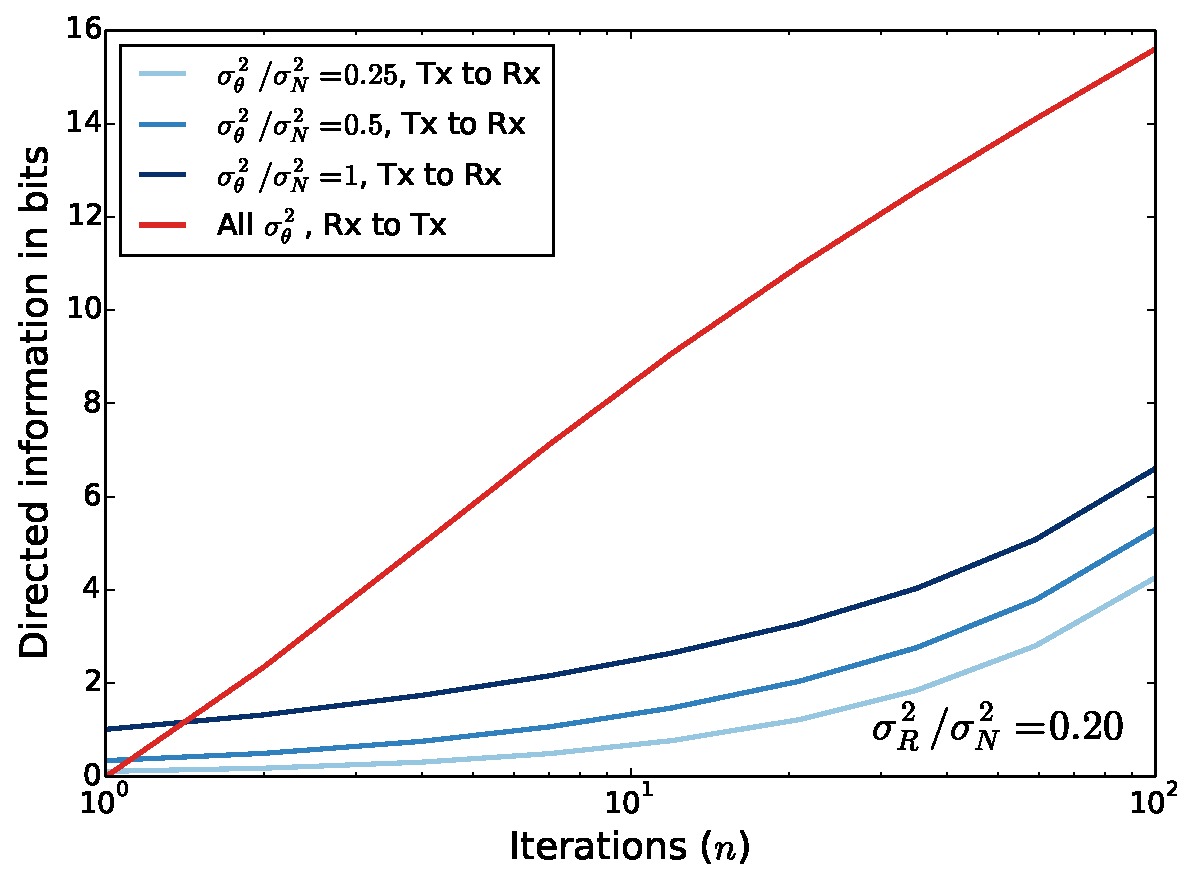
\includegraphics[width=3.2in]{noisy-fb-sigma_r2-point20} \\
	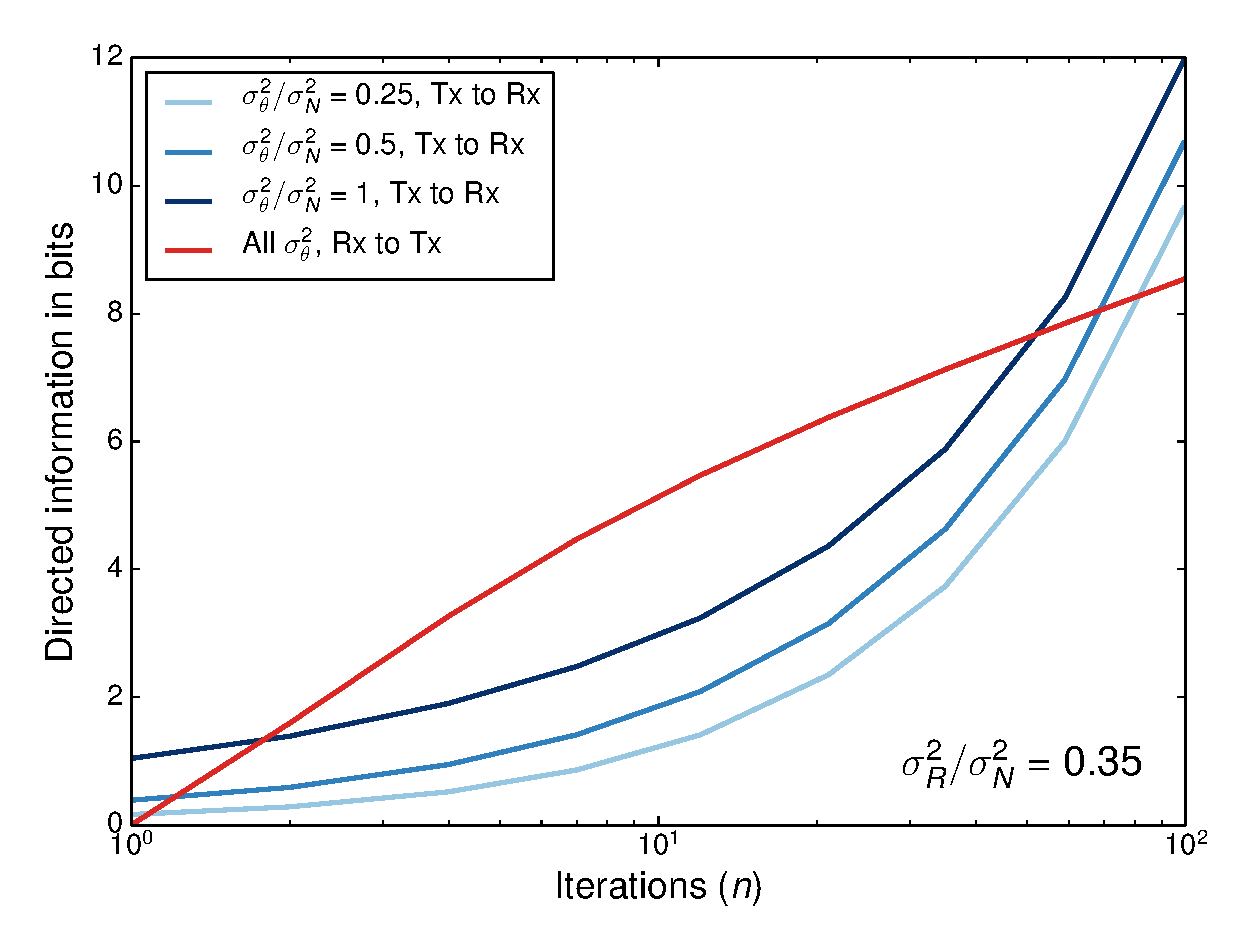
\includegraphics[width=3.2in]{noisy-fb-sigma_r2-point35} \\
	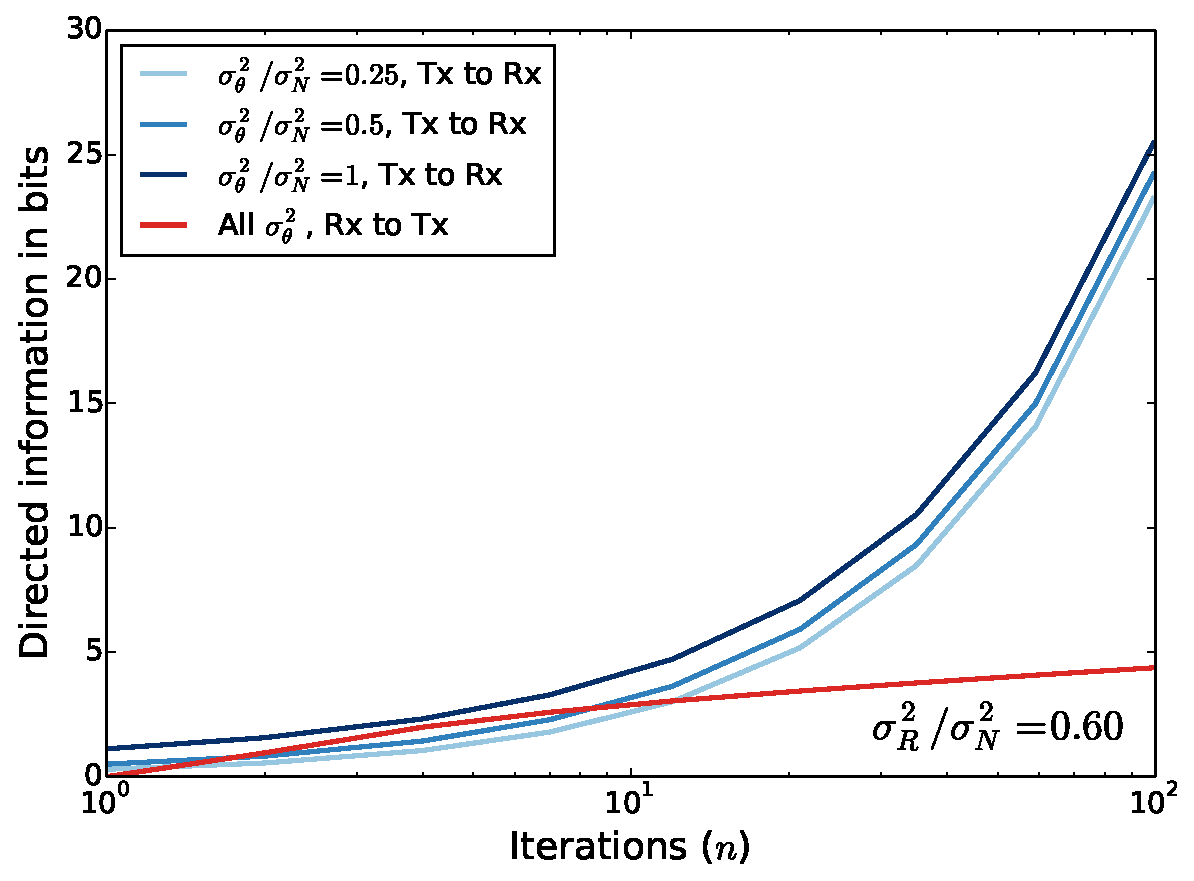
\includegraphics[width=3.2in]{noisy-fb-sigma_r2-point60}
	\caption{Plots for forward and backward directed information computations for ${\sigma_R^2}/{\sigma_N^2}=0.2$ (top), $0.35$ (center) and $0.6$ (bottom). In each plot, curves for directed information in both directions are illustrated for ratios ${\sigma_\theta^2}/{\sigma_N^2} = 0.25, 0.5,$ and $1$. The x-axis is the number of iterations of message-passing between the transmitter and the receiver. For cases when feedback noise variance $\sigma_R^2$ is moderately smaller than feedforward noise variance $\sigma_N^2$, directed information in the reverse link can dominate that in the forward link. With sufficiently many (albeit sometimes large, as illustrated in the top figure) iterations, directed information in forward information starts to dominate. However, the point at which this happens depends on the (often unknown) ratio of noise in these links. }
		     \label{fig:numerical}
\end{figure}

\section{Conclusions and discussions}
\label{sec:conclusions}

%%%%%%%%%%%%%%%%%%
There are several shortcomings of this work that need to be addressed for a more comprehensive understanding of the issue. First, our information source does not evolve with time, and hence our communication process (inspired from the scheme of Schalkwijk and Kailath~\cite{S&K} is non-ergodic. Since Granger causality is really just relative errors in prediction of a process, in presence or absence of knowledge of another process, we compute the obvious generalization of Granger causality to non-ergodic processes. Nevertheless, future work will address a situation with a linear dynamical system as the information source. Second, our experiments restrict themselves to Gaussian noise for simplicity, but neural spiking and spike-rate models for spikes tend to be very different from those used here. This is a clear direction for future work. Third, the power and energy constraints are somewhat oversimplified to make the analysis simpler. This is for simplicity of exposition. A more general analysis is a trivial extension. Finally, we consider a simple point-to-point network. In general networks, this issue could be even more complex. However, since this issue shows up even for the simplest network, we feel that the problem will only be exacerbated when the network is large.

We note that Granger's original analysis does not compare Granger causality on forward and reverse links. We are doing so, in part because it is often done in practice. It strikes us that this is being done because of the ``conservation of directed information'', an equality first derived by Massey~\cite{massey2005conservation}. This equality, which states that the sum of forward and reverse Directed Informations is the mutual information, could be viewed as suggesting that an increase in Directed Information in one direction must reduce it in the other direction. However, this is not true. For e.g., making $X$ and $Y$ uncorrelated reduces Directed Information in both directions (along with their sum) to zero. In other words, Massey's law is not a conservation law in the sense of conservation laws of energy, momentum, or mass, where the total energy/momentum/mass (\textit{i.e.}, the RHS) remains conserved (\textit{i.e.}, constant) regardless of the experiment performed on the entities.

\section*{Acknowledgments}


The authors would like to thank Nicola Elia for discussions that suggested this possible misunderstanding in use of Granger causality and Directed Information in computational systems. Praveen Venkatesh is partially supported by a dean's fellowship. %Pulkit Grover is supported by [...].


\bibliographystyle{IEEEtran}
\bibliography{IEEEabrv,references}


\newpage

\appendices

\section{Directed Information in the forward direction, noiseless feedback}
\label{app:appendix3}

The Directed Information in the forward direction is computed as:
\begin{align*}
	I(X^n \rightarrow \widehat\Theta^n) &= \sum_{i=1}^n{I(\widehat\Theta_i ; X^i | \widehat\Theta^{i-1})} \\
										&= \sum_{i=1}^n{h(\widehat\Theta_i | \widehat\Theta^{i-1}) - h(\widehat\Theta_i | \widehat\Theta^{i-1}, X^i)} \numberthis \label{eq:dir-info-fwd-noiseless}
\end{align*}
Taking the first term in \eqref{eq:dir-info-fwd-noiseless},
\begin{align*}
	h(\widehat\Theta_i | \widehat\Theta^{i-1}) &= h \bigg( \widehat\Theta_{i-1} + \frac{X_i + N_i}{i} \bigg| \widehat\Theta^{i-1} \bigg) \\
											   &= h(\Theta - \widehat\Theta_{i-1} + N_i | \widehat\Theta^{i-1}) -\log(i) \\
											   &= h(\Theta + N_i | \widehat\Theta^{i-1}) -\log(i) \\
											   &= h(\Theta + N_i | \widehat\Theta_{i-1}) -\log(i)
\end{align*}
where we have dropped the conditioning on all except $\widehat\Theta_{i-1}$ in the last step. %TODO: Justify. Markov proof is too long to write here.
Define $U = \Theta + N_i$ and $V = \widehat\Theta_{i-1}$. Since all variables are Gaussian, it suffices to find the variance of the conditional distribution $U|V$.
\begin{align*}
	\mathbb{E}[U] = 0,
	\mathbb{E}[V] &= 0, \text{Var}[U] = \sigma_\theta^2 + \sigma_N^2,
	\text{Var}[V] = \sigma_\theta^2+ \frac{\sigma_N^2}{i-1} \\
	\text{Cov}[U,V] &= \mathbb{E}[UV]-\mathbb{E}[U]\mathbb{E}[V] \\
					&= \sigma_\theta^2 \\
	\rho^{2}        &= \frac{\sigma_{\theta}^{4}}{(\sigma_{\theta}^{2}+\sigma_{N}^{2})(\sigma_{\theta}^{2}+\frac{\sigma_{N}^{2}}{(i-1)})}
\end{align*}
\begin{equation*}
	U|V=v\ \sim\ \mathcal{N}\left(\sqrt{\frac{\sigma_{\theta}^{2}+\sigma_{N}^{2}}{\sigma_{\theta}^{2}+\frac{\sigma_{N}^{2}}{i-1}}}\rho v,(1-\rho^{2})(\sigma_{\theta}^{2}+\sigma_{N}^{2})\right)
\end{equation*}
Hence, the entropy of the conditional distribution is
\begin{equation*}
	h(U|V=v)=\frac{1}{2}\log(2\pi e(1-\rho^{2})(\sigma_{\theta}^{2}+\sigma_{N}^{2})) \overset{(a)}{=} h(U|V)
\end{equation*}
where (a) follows because the conditional entropy is independent of $v$. Thus,
\begin{equation}
	h(\widehat{\Theta}_{i}|\widehat{\Theta}^{i-1}) = \frac{1}{2}\log\left(2\pi e\frac{\sigma_{N}^{2}(i\sigma_{\theta}^{2}+\sigma_{N}^{2})}{((i-1)\sigma_{\theta}^{2}+\sigma_{N}^{2})}\right)-\log(i) \label{eq:htheta_theta-noiseless}
\end{equation}
The next term in equation \eqref{eq:dir-info-fwd-noiseless} is
\begin{align*}
	h(\widehat{\Theta}_{i}|\widehat{\Theta}^{i-1},X^{i}) &= h\left(\frac{N_{i}}{i}\bigg|\widehat{\Theta}^{i-1},X^{i}\right) \\
												 &= h(N_{i}) -\log(i) \\
												 &= \frac{1}{2}\log(2\pi e\sigma_{N}^{2}) -\log(i) \numberthis \label{eq:htheta_x_theta-noiseless}
\end{align*}
Putting equations \eqref{eq:htheta_theta-noiseless} and \eqref{eq:htheta_x_theta-noiseless} together, we can compute the forward Directed Information:
\begin{align*}
	I(\widehat{\Theta}_{i};X^{i}|\widehat{\Theta}^{i-1}) &= h(\widehat{\Theta}_{i}|\widehat{\Theta}^{i-1}) - h(\widehat{\Theta}_{i}|\widehat{\Theta}^{i-1},X^{i}) \\
	                                             &= \frac{1}{2}\log\left(\frac{i\sigma_{\theta}^{2}+\sigma_{N}^{2}}{(i-1)\sigma_{\theta}^{2}+\sigma_{N}^{2}}\right) \\
	I(X^{n} \rightarrow \widehat{\Theta}^{n})    &= \sum_{i=1}^{n}I(\widehat{\Theta}_{i};X^{i}|\widehat{\Theta}^{i-1}) \\
												 &\overset{(a)}{=} \frac{1}{2}\log\left(\frac{n\sigma_{\theta}^{2}+\sigma_{N}^{2}}{\sigma_{N}^{2}}\right) \\
	                                             &= \frac{1}{2}\log\left(1+\frac{n\sigma_{\theta}^{2}}{\sigma_{N}^{2}}\right)
\end{align*}
where (a) follows through by expanding out the product inside the logarithms and canceling terms. Clearly, this value is finite.

\section{Directed Information in the forward direction, with noisy feedback}
\label{app:appendix1}

\begin{align*}
	I(X^n \rightarrow \widehat\Theta^n) &= \sum_{i=1}^n{I(\widehat\Theta_i ; X^i | \widehat\Theta^{i-1})} \\
									 &= \sum_{i=1}^n{h(\widehat\Theta_i | \widehat\Theta^{i-1}) - h(\widehat\Theta_i | \widehat\Theta^{i-1}, X^i)}
\end{align*}
Taking the first of the two terms in the above expression,
\begin{align*}
	h(\widehat\Theta_i | \widehat\Theta^{i-1}) &\overset{(a)}{=} h(\widehat\Theta_{i-1} \frac{i-1}{i} + \frac{\Theta}{i} - \frac{R_{i-1}}{i} + \frac{N_i}{i} | \widehat\Theta^{i-1}) \\
											   &= h(\Theta - R_{i-1} + N_i | \widehat\Theta^{i-1}) -\log(i)
\end{align*}
where for (a) we have used equation \eqref{eq:theta_hat_i-noisy-once}. The Markov property no longer holds in this case, but we proceed in the same manner. We define $U = \Theta - R_{i-1} + N_i$ and $\underbar{V} = \widehat\Theta^{i-1}$. Recalling equation \eqref{eq:theta_hat_i-noisy}, for $j \in \{1, \ldots i-1\}$, $p \in \{1, \ldots i-1\}$ and $q \in \{1, \ldots i-1\}$, we have
\begin{align*}
	\mathbb{E}[U] &= 0,\;	\mathbb{E}[\widehat\Theta_j] = 0,\;\\	\mathbb{E}[U^2] &= \sigma_\theta^2 + \sigma_R^2 + \sigma_N^2,\;	\mathbb{E}[U \widehat\Theta_j] = \sigma_\theta^2 \\
	\mathbb{E}[\widehat\Theta_p \widehat\Theta_q] &= \mathbb{E} \bigg[ \bigg( \Theta + \frac{1}{p} \sum_{k=1}^p N_k - \frac{1}{p} \sum_{k=1}^{p-1} R_k \bigg)\\
												  & \qquad \qquad \bigg( \Theta + \frac{1}{q} \sum_{k=1}^q N_k - \frac{1}{q} \sum_{k=1}^{q-1} R_k \bigg) \bigg] \\
												  &= \sigma_\theta^2 + \frac{\min\{p, q\}}{pq} \sigma_N^2 + \frac{\min\{p-1, q-1\}}{pq} \sigma_R^2 \\
	\text{Var}[U|\widehat\Theta^{i-1}] &= \mathbb{E}[U^2] - \mathbb{E}[U \underbar{V}] \mathbb{E}[\underbar{V} \underbar{V}^T]^{-1} \mathbb{E}[\underbar{V} U] \\
	h(U | \widehat\Theta^{i-1}) &= \frac{1}{2}\log(2 \pi e \text{Var}[U | \widehat\Theta^{i-1}]) \numberthis \label{eq:h_theta_theta-noisy}
\end{align*}
We can not derive a simple closed form for this expression, but we have computed it numerically for the plots in Section~\ref{sec:numerical-results}. The second term in equation \eqref{eq:dir-info-fwd-noisy} is
\begin{align*}
	h(\widehat\Theta_i | \widehat\Theta^{i-1}, X^i) &= h \bigg( \widehat\Theta_{i-1} + \frac{X_i + N_i}{i} \bigg| \widehat\Theta^{i-1}, X^i \bigg) \\
													&= h(N_i | \widehat\Theta^{i-1}, X^i) -\log(i) \\
													&= \frac{1}{2}\log(2 \pi e \sigma_N^2) -\log(i) \numberthis \label{eq:h_theta_x_theta-noisy}
\end{align*}
From equations \eqref{eq:h_theta_theta-noisy} and \eqref{eq:h_theta_x_theta-noisy}, we compute the forward-directed information as depicted in Section~\ref{sec:numerical-results}, for different values of $\sigma_\theta^2$.

% you can choose not to have a title for an appendix
% if you want by leaving the argument blank
\section{Directed Information in the reverse direction, with noisy feedback}
\label{app:appendix2}

\begin{align*}
	I(0*\widehat\Theta^{n-1} \rightarrow X^n) &= \sum_{i=0}^{n-1}{I(X_{i+1}; \widehat\Theta^i | X^i)} \\
											  &= \sum_{i=0}^{n-1}{h(X_{i+1} | X^i) - h(X_{i+1} | X^i, \widehat\Theta^i)} \numberthis \label{eq:dir-info-rev-noisy}
\end{align*}
Taking the first term inside the summation,
\begin{align*}
	h(X_{i+1} | X^i) &= h(\Theta - \widehat\Theta_i - R_i | X^i) \\
					&\overset{(a)}{=} h \bigg( \bigg( - \widehat\Theta_{i-1} - \frac{X_i + N_i}{i} \bigg) - R_i \bigg| X^i \bigg) \\
					&\overset{(b)}{=} h \bigg( \bigg( X_i - \Theta + R_{i-1} - \frac{N_i}{i} \bigg) - R_i \bigg| X^i \bigg) \\
					&\overset{(c)}{=} h \bigg( R_{i-1} - \frac{N_i}{i} - R_i \bigg| X^i \bigg)
\end{align*}
where in (a) above, we have dropped $\Theta = X_1$, in (b) we have re-expressed $\widehat\Theta_{i-1}$ in terms of $X_i$, $\Theta$ and $R_{i-1}$, and in (c) we have dropped $X_i$ and $\Theta$ again. As before, define $U = R_{i-1} - \frac{N_i}{i} - R_i$, so that
\begin{equation*}
	\mathbb{E}[U] = 0,\; \; \mathbb{E}[X_j] = 0, \; \; \mathbb{E}[U^2] = 2 \sigma_R^2 + \frac{\sigma_N^2}{i^2}
\end{equation*}
For $i \geq 3$ and $j \in \{3, \ldots i\}$, we can use equation \eqref{eq:x_i-noisy} to see that
\begin{align*}
	\mathbb{E}[U X_j] &= \mathbb{E} \bigg[ \bigg( R_{i-1} - \frac{N_i}{i} - R_i \bigg) \\
					  & \qquad             \bigg( \frac{1}{j-1} \sum_{k=1}^{j-2} R_k - \frac{1}{j-1} \sum_{k=1}^{j-1} N_k - R_{j-1} \bigg) \bigg] \\
					  &= - \mathbb{E}[R_{i-1} R_{j-1}] = - \sigma_R^2 \delta_{ij} \\
	\mathbb{E}[U X_1] &= \mathbb{E} \bigg[ \bigg( R_{i-1} - \frac{N_i}{i} - R_i \bigg) \Theta \bigg] = 0 \; \\
	\mathbb{E}[U X_2] &= \mathbb{E} \bigg[ \bigg( R_{i-1} - \frac{N_i}{i} - R_i \bigg) (\Theta - (\Theta + N_i) - R_1) \bigg] = 0 \; \\
	\mathbb{E}[X_p X_q] &= \mathbb{E} \bigg[ \bigg( \frac{1}{p-1} \sum_{k=1}^{p-2} R_k - \frac{1}{p-1} \sum_{k=1}^{p-1} N_k - R_{p-1} \bigg) \\
						& \qquad             \bigg( \frac{1}{q-1} \sum_{k=1}^{q-2} R_k - \frac{1}{q-1} \sum_{k=1}^{q-1} N_k - R_{q-1} \bigg) \bigg] \\
					    &= \frac{\min\{p-2, q-2\}}{(p-1)(q-1)} \sigma_R^2 + \frac{\min\{p-1, q-1\}}{(p-1)(q-1)} \sigma_N^2 \\
						& \qquad + \sigma_R^2 \delta_{pq} + \frac{1}{p-1} \sigma_R^2 \mathbb{I}_{p>q} + \frac{1}{q-1} \sigma_R^2 \mathbb{I}_{q>p} \\
	\mathbb{E}[X_1 X_1] &= \mathbb{E}[\Theta^2] = \sigma_\theta^2 \\
	\mathbb{E}[X_1 X_j] &= \mathbb{E} \bigg[ \Theta \bigg( \frac{1}{j-1} \sum_{k=1}^{j-2} R_k - \frac{1}{j-1} \sum_{k=1}^{j-1} N_k - R_{j-1} \bigg) \bigg] = 0 \\
	\text{Var}[U|X^i] &= \mathbb{E}[U^2] - \mathbb{E}[U X^i] \mathbb{E}[X^i {X^i}^T]^{-1} \mathbb{E}[X^i U] \\
	h(U | X^i) &= \frac{1}{2}\log(2 \pi e \text{Var}[U | X^i]) \numberthis \label{eq:h_x_x-noisy}
\end{align*}
The above argument can be extended to $i=2$ by letting the final index of the summation term be smaller than the starting index, implying that the whole summation term is simply dropped. The special cases of $i=0$ and $i=1$ are handled at the end. The second term from equation \eqref{eq:dir-info-rev-noisy} becomes
\begin{align*}
	h(X_{i+1} | X^i, \widehat\Theta^i) &= h(\Theta - \widehat\Theta_i - R_i | X^i, \widehat\Theta^i) \\
									   &= \frac{1}{2}\log(2 \pi e \sigma_R^2) \numberthis \label{eq:h_x_x_theta-noisy}
\end{align*}
because $X_1 = \Theta$ and because $R_i$ is independent of all the $X^i$ and $\widehat\Theta^i$. For the special cases of $i=0$ and $i=1$, we solve for the value of mutual information explicitly:
\begin{align*}
	i = 0: & \qquad I(X_1; \widehat\Theta^0 | X^0) &=& \; h(X_1) - h(X_1) = 0 \\
	i = 1: & \qquad I(X_2; \widehat\Theta^1 | X^1) &=& \; h(X_2 | X_1) - h(X_2 | X_1, \widehat\Theta_1) \\
		   & \qquad h(X_2 | X_1)                   &=& \; h(\Theta - \widehat\Theta_1 - R_1 | X^1) \\
		   & \qquad                                &=& \; h(-\Theta - N_1 - R_1 | X_1) \\
		   & \qquad                                &=& \; h(-N_1 - R_1) \\
		   & \qquad                                &=& \; \frac{1}{2} \log(2 \pi e (\sigma_N^2 + \sigma_R^2)) \\
		   & \qquad h(X_2 | X_1, \widehat\Theta_1) &=& \; h(-R_1) = \frac{1}{2} \log(2 \pi e \sigma_R^2) \\
		   & \qquad I(X_2; \widehat\Theta^1 | X^1) &=& \; \frac{1}{2} \log \bigg( 2 \pi e \frac{\sigma_N^2 + \sigma_R^2}{\sigma_R^2} \bigg)
\end{align*}
From equations \eqref{eq:h_x_x-noisy} and \eqref{eq:h_x_x_theta-noisy}, along with the two special cases above, we can now compute the reverse-directed information plotted in Section~\ref{sec:numerical-results}.




% trigger a \newpage just before the given reference
% number - used to balance the columns on the last page
% adjust value as needed - may need to be readjusted if
% the document is modified later
%\IEEEtriggeratref{14}
% The "triggered" command can be changed if desired:
%\IEEEtriggercmd{\enlargethispage{-5in}}

% references section

% can use a bibliography generated by BibTeX as a .bbl file
% BibTeX documentation can be easily obtained at:
% http://www.ctan.org/tex-archive/biblio/bibtex/contrib/doc/
% The IEEEtran BibTeX style support page is at:
% http://www.michaelshell.org/tex/ieeetran/bibtex/
%\bibliographystyle{IEEEtran}
% argument is your BibTeX string definitions and bibliography database(s)
%\bibliography{IEEEabrv,../bib/paper}
%
% <OR> manually copy in the resultant .bbl file
% set second argument of \begin to the number of references
% (used to reserve space for the reference number labels box)




% that's all folks
\end{document}


